%%%%%%%%%%%%%%%%%%%%%%%%%%%%%%%%%%%%%%%%%
% Beamer Presentation
% LaTeX Template
% Version 1.0 (10/11/12)
%
% This template has been downloaded from:
% http://www.LaTeXTemplates.com
%
% License:
% CC BY-NC-SA 3.0 (http://creativecommons.org/licenses/by-nc-sa/3.0/)
%
%%%%%%%%%%%%%%%%%%%%%%%%%%%%%%%%%%%%%%%%%

%----------------------------------------------------------------------------------------
%	PACKAGES AND THEMES
%----------------------------------------------------------------------------------------

\documentclass[UTF8,aspectratio=169,14pt]{ctexbeamer}

\usepackage{hyperref}
\hypersetup{
	colorlinks=true,
	linkcolor=red,
	anchorcolor=blue,
	citecolor=green
}

\mode<presentation> {
	
	% The Beamer class comes with a number of default slide themes
	% which change the colors and layouts of slides. Below this is a list
	% of all the themes, uncomment each in turn to see what they look like.
	
	%\usetheme{default}
	%\usetheme{AnnArbor}
	%\usetheme{Antibes}
	%\usetheme{Bergen}
	%\usetheme{Berkeley}
	%\usetheme{Berlin}
	%\usetheme{Boadilla}
	%\usetheme{CambridgeUS}
	%\usetheme{Copenhagen}
	%\usetheme{Darmstadt}
	%\usetheme{Dresden}
	%\usetheme{Frankfurt}
	%\usetheme{Goettingen}
	%\usetheme{Hannover}
	%\usetheme{Ilmenau}
	%\usetheme{JuanLesPins}
	%\usetheme{Luebeck}
	\usetheme{Madrid}
	%\usetheme{Malmoe}
	%\usetheme{Marburg}
	%\usetheme{Montpellier}
	%\usetheme{PaloAlto}
	%\usetheme{Pittsburgh}
	%\usetheme{Rochester}
	%\usetheme{Singapore}
	%\usetheme{Szeged}
	%\usetheme{Warsaw}
	
	% As well as themes, the Beamer class has a number of color themes
	% for any slide theme. Uncomment each of these in turn to see how it
	% changes the colors of your current slide theme.
	
	%\usecolortheme{albatross}
	%\usecolortheme{beaver}
	%\usecolortheme{beetle}
	%\usecolortheme{crane}
	%\usecolortheme{dolphin}
	%\usecolortheme{dove}
	%\usecolortheme{fly}
	%\usecolortheme{lily}
	%\usecolortheme{orchid}
	%\usecolortheme{rose}
	%\usecolortheme{seagull}
	%\usecolortheme{seahorse}
	%\usecolortheme{whale}
	%\usecolortheme{wolverine}
	
	%\setbeamertemplate{footline} % To remove the footer line in all slides uncomment this line
	%\setbeamertemplate{footline}[page number] % To replace the footer line in all slides with a simple slide count uncomment this line
	
	%\setbeamertemplate{navigation symbols}{} % To remove the navigation symbols from the bottom of all slides uncomment this line
}

\usepackage{graphicx} % Allows including images
\graphicspath{{./figs/}}
\usepackage{booktabs} % Allows the use of \toprule, \midrule and \bottomrule in tables
\usepackage{longtable}
\usepackage{listings}
\usepackage{xcolor}
\lstset{numbers=left, %设置行号位置
	numberstyle=\tiny, %设置行号大小
	keywordstyle=\color{blue}, %设置关键字颜色
	commentstyle=\color[cmyk]{1,0,1,0}, %设置注释颜色
	frame=single, %设置边框格式
	escapeinside=``, %逃逸字符(1左面的键),用于显示中文
	%breaklines, %自动折行
	extendedchars=false, %解决代码跨页时,章节标题,页眉等汉字不显示的问题
	xleftmargin=2em,xrightmargin=2em, aboveskip=1em, %设置边距
	tabsize=4, %设置tab空格数
	showspaces=false %不显示空格
}
% Fonts
% \usepackage{libertine}
% \setmonofont{Courier}
\setCJKsansfont[ItalicFont=Noto Serif CJK SC Black, BoldFont=Noto Sans CJK SC Black]{Noto Sans CJK SC}


%----------------------------------------------------------------------------------------
%	TITLE PAGE
%----------------------------------------------------------------------------------------

\title[第2讲]{第2讲 :操作系统与系统结构和程序设计语言} % The short title appears at the bottom of every slide, the full title is only on the title page
\subtitle{第一节:从OS角度看计算机系统}
\author{向勇、陈渝} % Your name
\institute[清华大学] % Your institution as it will appear on the bottom of every slide, may be shorthand to save space
{
清华大学计算机系 \\ % Your institution for the title page
\medskip
\textit{xyong,yuchen@tsinghua.edu.cn} % Your email address
}
\date{\today} % Date, can be changed to a custom date

\begin{document}

\begin{frame}
\titlepage % Print the title page as the first slide
\end{frame}

\begin{frame}
\frametitle{提纲} % Table of contents slide, comment this block out to remove it
\tableofcontents % Throughout your presentation, if you choose to use \section{} and \subsection{} commands, these will automatically be printed on this slide as an overview of your presentation
\end{frame}

%----------------------------------------------------------------------------------------
%	PRESENTATION SLIDES
%----------------------------------------------------------------------------------------

%------------------------------------------------
\section{第一节:从OS角度看计算机系统 } % Sections can be created in order to organize your presentation into discrete blocks, all sections and subsections are automatically printed in the table of contents as an overview of the talk
%------------------------------------------------

\subsection{隔离} % A subsection can be created just before a set of slides with a common theme to further break down your presentation into chunks

\begin{frame}

\frametitle{再看计算机系统}

\begin{figure}
	\centering
	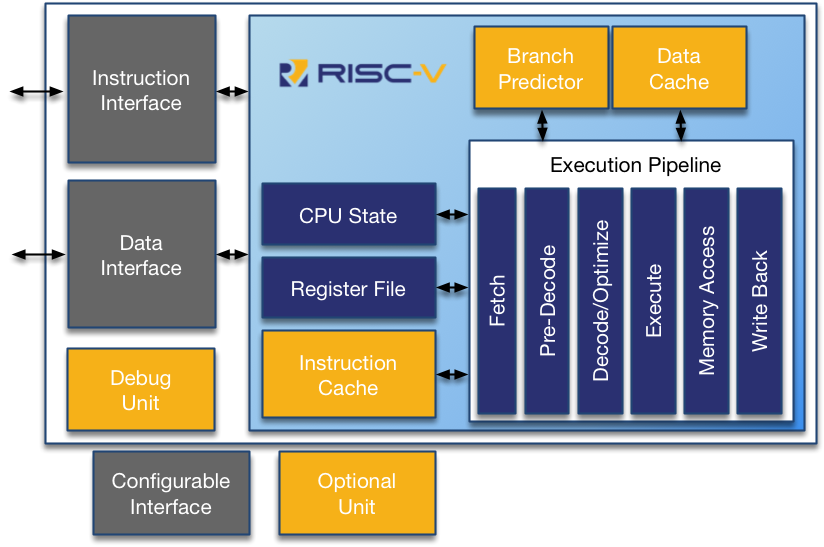
\includegraphics[width=0.45\linewidth]{rv-arch}
	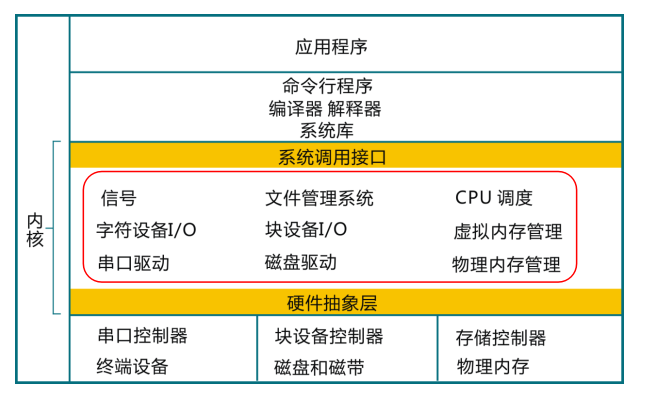
\includegraphics[width=0.45\linewidth]{ucore-arch}	
	\caption{再看计算机系统 -- 从OS角度}
\end{figure}


\end{frame}




\begin{frame}
	\frametitle{隔离:\small{程序调用}}
	\begin{itemize}
		\item 程序调用 \textit{ssize\_t read(int fd, void *buf, size\_t count);}会发生什么?
		\item 我们可以在应用程序中直接调用内核的函数吗?
		\item 我们可以在内核中使用应用程序普通的函数调用吗? \pause
		\item 程序调用的特征
		\begin{itemize}
			\item 好处:执行很快;
			\item 好处:灵活-易于传递和返回复杂数据类型;
			\item 好处:程序员熟悉的机制,...
			\item 坏处:应用程序不可靠,可能有恶意,有崩溃的风险
			
		\end{itemize}
	\end{itemize}
\end{frame}



\begin{frame}
	\frametitle{隔离:\small{什么是隔离?}}
%	\begin{itemize}
%		\item 什么是隔离?
		\begin{itemize}

		\item 强制隔离以避免对整个系统的可用性/可靠性/安全影响
		\item 运行的程序通常是是隔离的单元
		\pause
		
		\item 防止程序X破坏或监视程序Y
			\begin{itemize}
			\item 读/写内存,使用100%的CPU,更改文件描述符
			\end{itemize}
		\item 防止进程干扰操作系统
		\item 防止恶意程序、病毒、木马和bug
			\begin{itemize}
			\item 错误的过程可能会试图欺骗硬件或内核
			\end{itemize}
		\end{itemize}
%	\end{itemize}
\end{frame}



\begin{frame}
	\frametitle{隔离:\small{主要的隔离方法?}}
%	\begin{itemize}
%		\item 主要的隔离方法?
		\begin{itemize}
			\item 地址空间 address spaces
				\begin{itemize}
				\item 一个程序仅寻址其自己的内存
				\item 每个程序若无许可,则无法访问不属于自己的内存
				\end{itemize}			
				\pause
			
			\item CPU硬件中的特权模式/中断机制
				\begin{itemize}
				\item 防止应用程序访问设备和敏感的CPU寄存器
				\item 例如地址空间配置寄存器
				\item 例如打断一直占用CPU的应用程序
				\end{itemize}				
		\end{itemize}
%	\end{itemize}
\end{frame}

\subsection{虚拟内存}

\begin{frame}[plain]
	
	\frametitle{虚拟内存}
	
	\begin{figure}
		\centering
		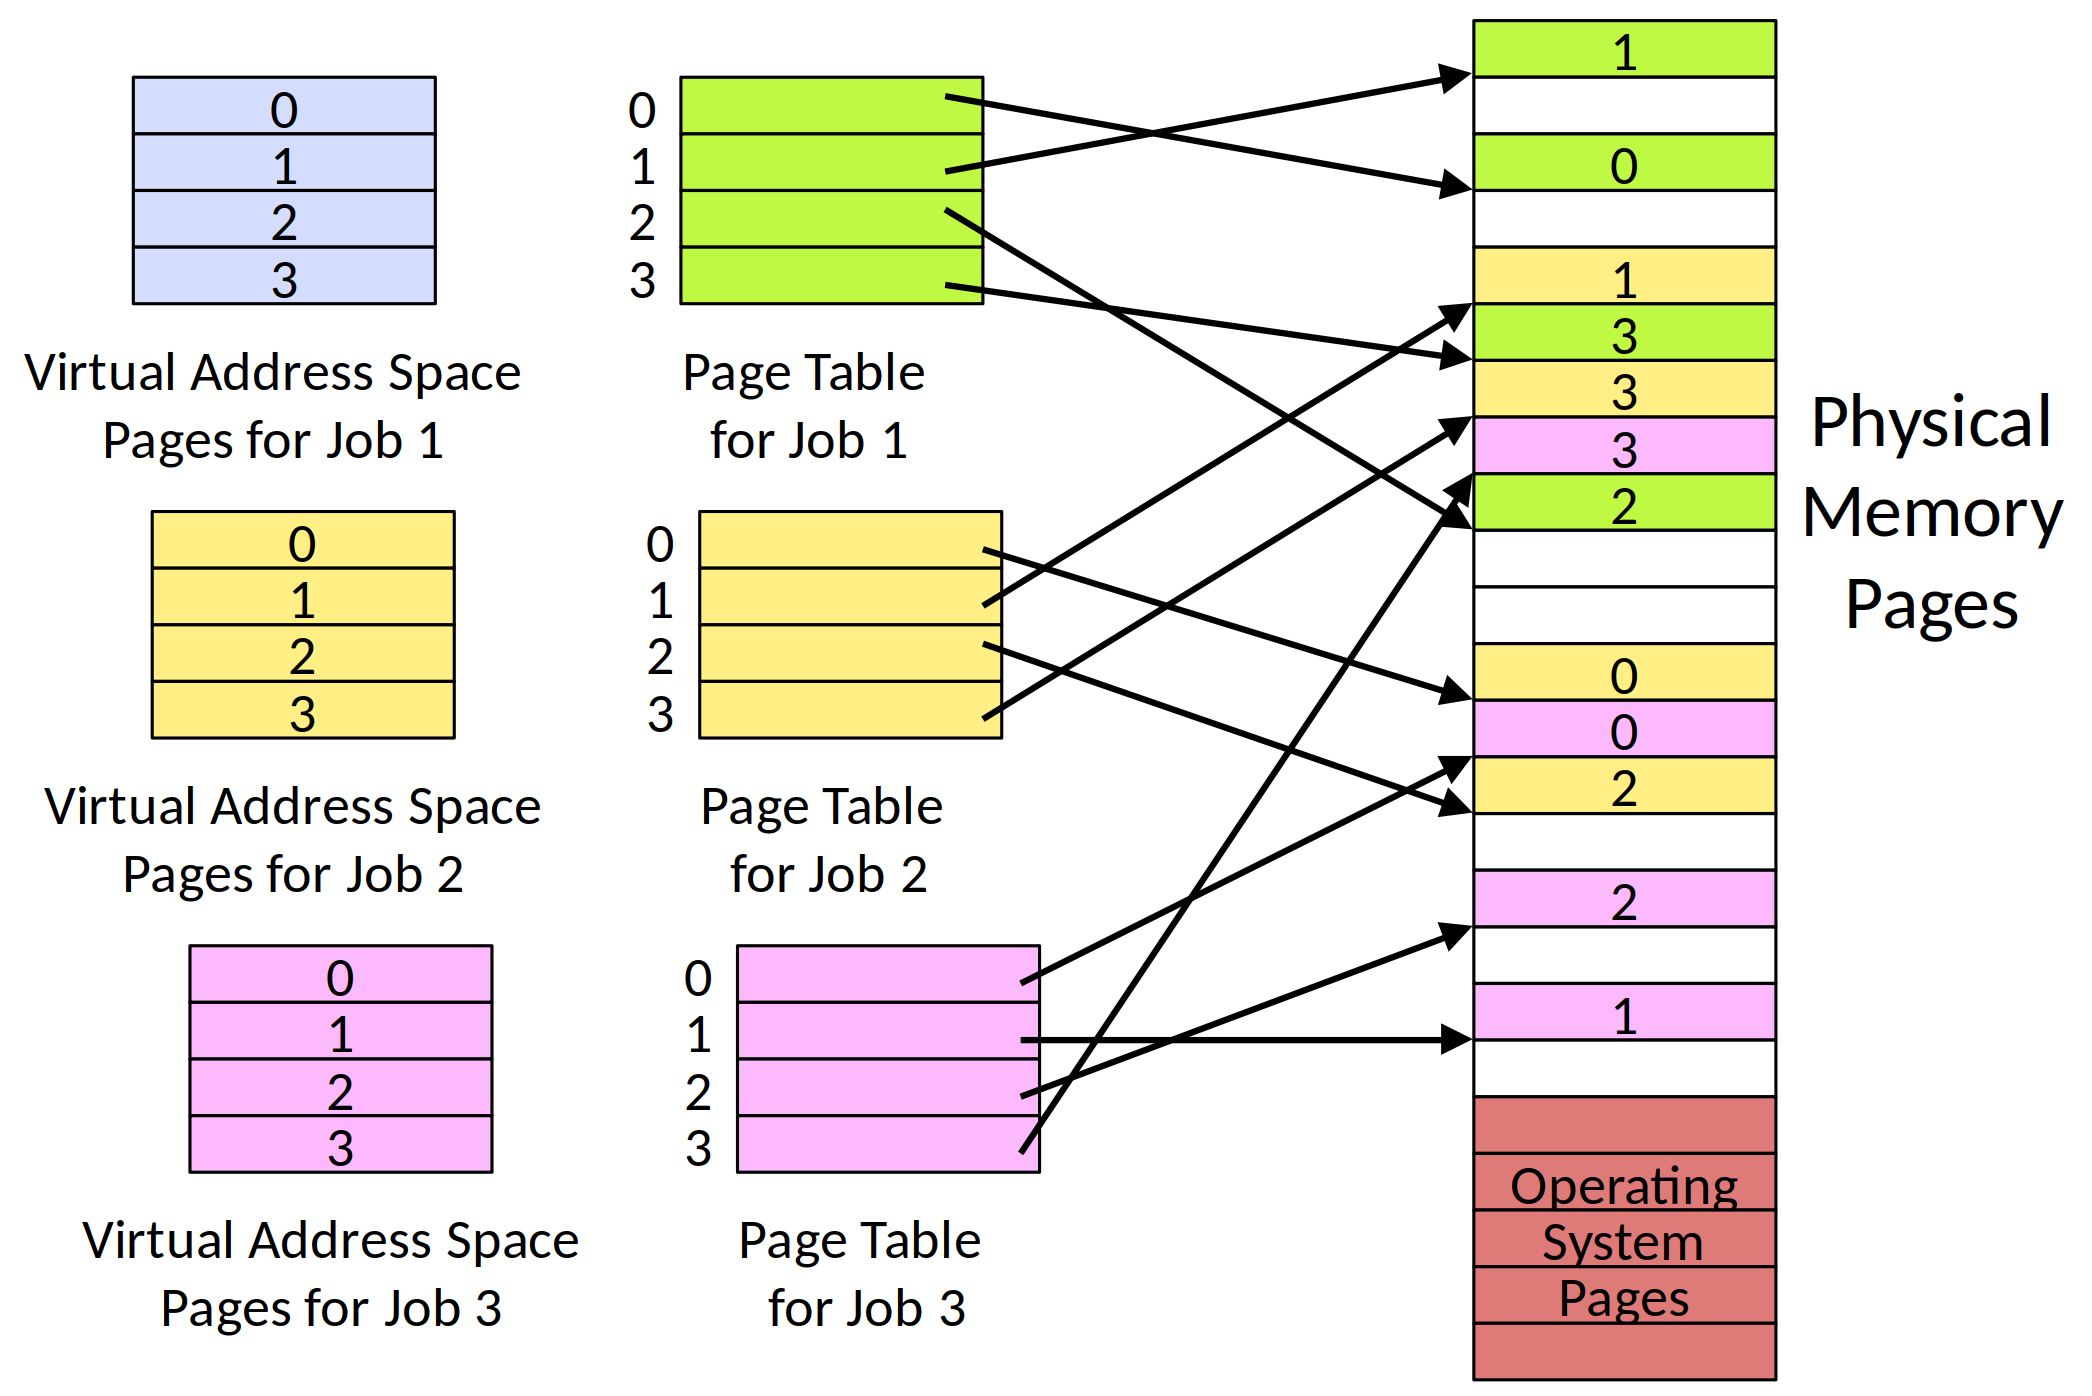
\includegraphics[width=0.65\linewidth]{vm}
		\caption{虚拟内存}
	\end{figure}
	% CS152-berkeley L08-AddressTranslation
	% 体系结构需要易于编程/编译/链接,易于软件管理	
	
\end{frame}

\begin{frame}[plain]
	
	\frametitle{虚拟内存}
	
	\begin{figure}
		\centering
		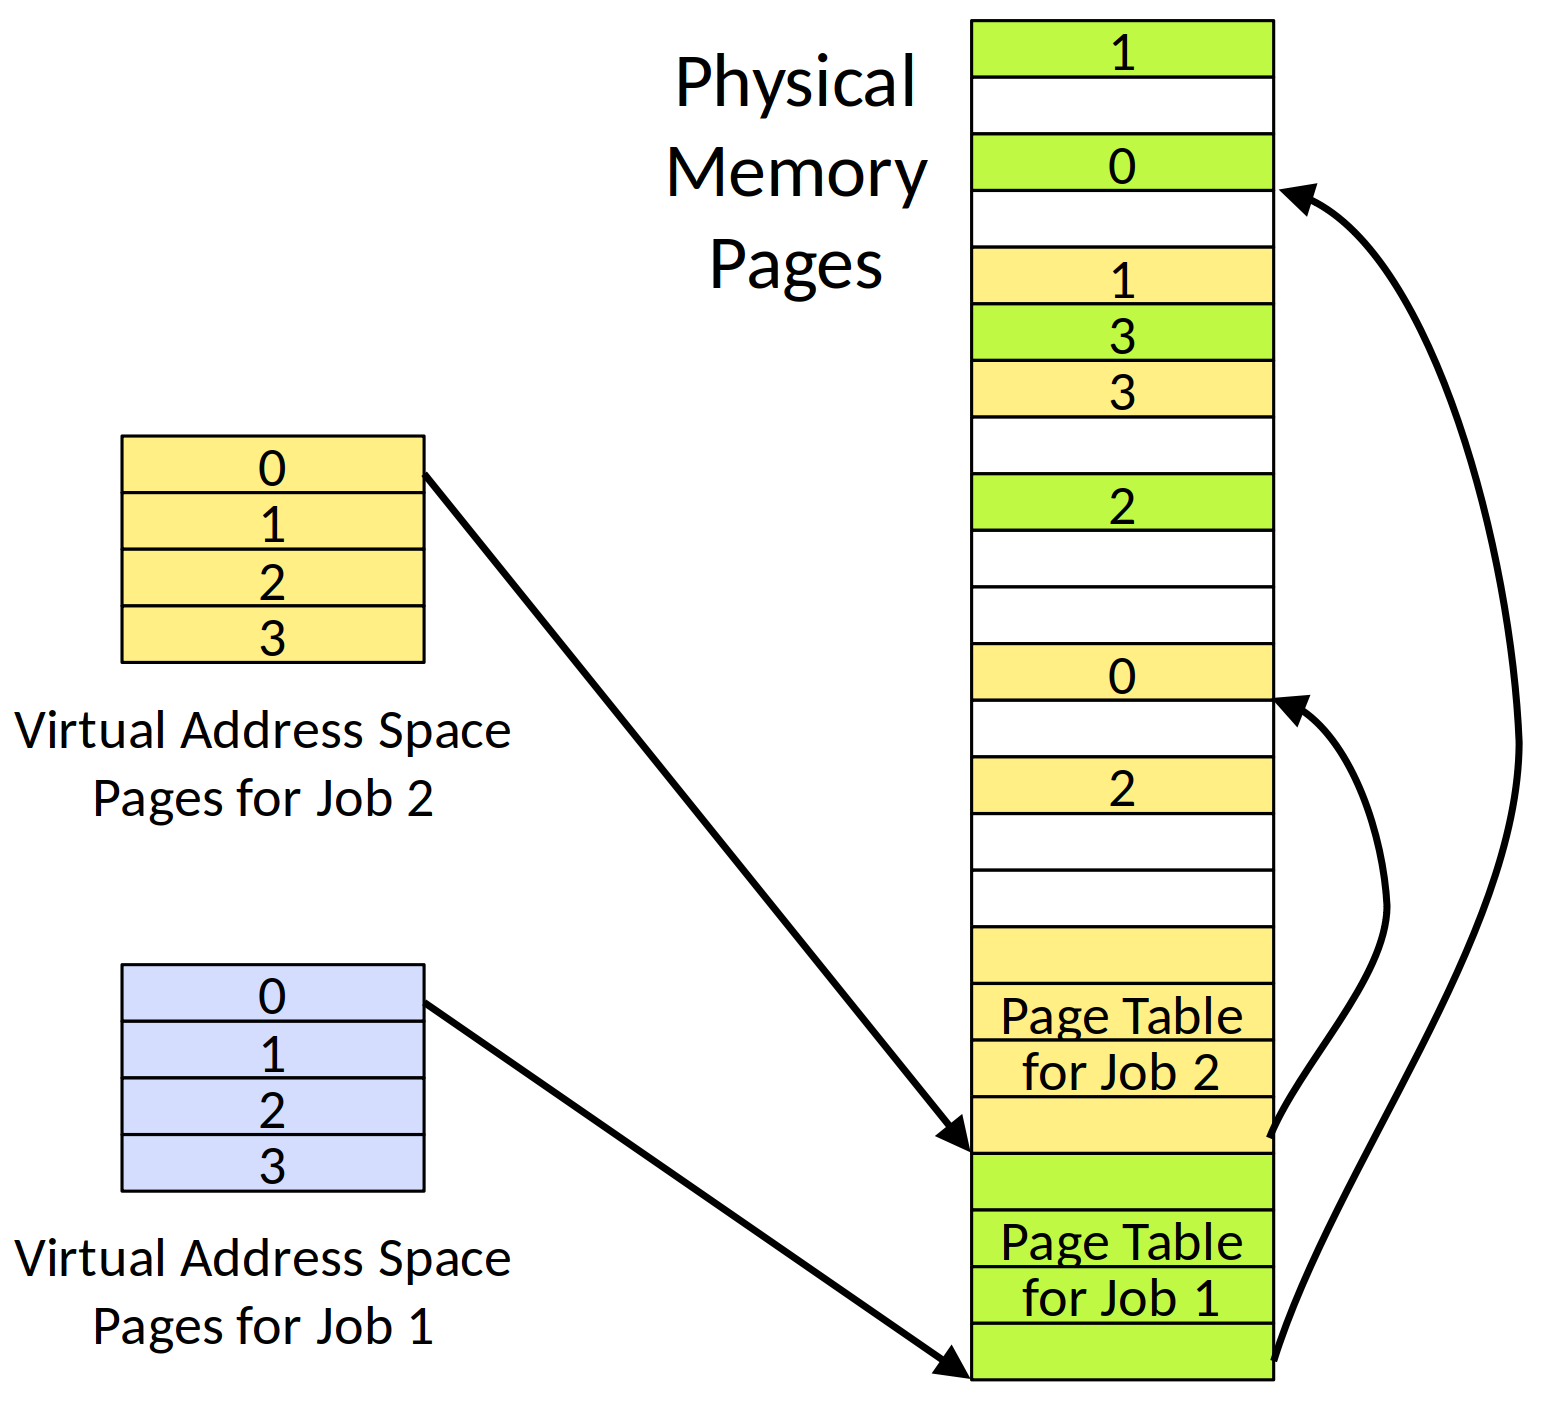
\includegraphics[width=0.5\linewidth]{vm-pagetable}
		\caption{页表}
	\end{figure}
	% CS152-berkeley
	% 体系结构需要易于编程/编译/链接,易于软件管理	
	
\end{frame}

\begin{frame}
	
	\frametitle{虚拟内存}
	
	\begin{figure}
		\centering
		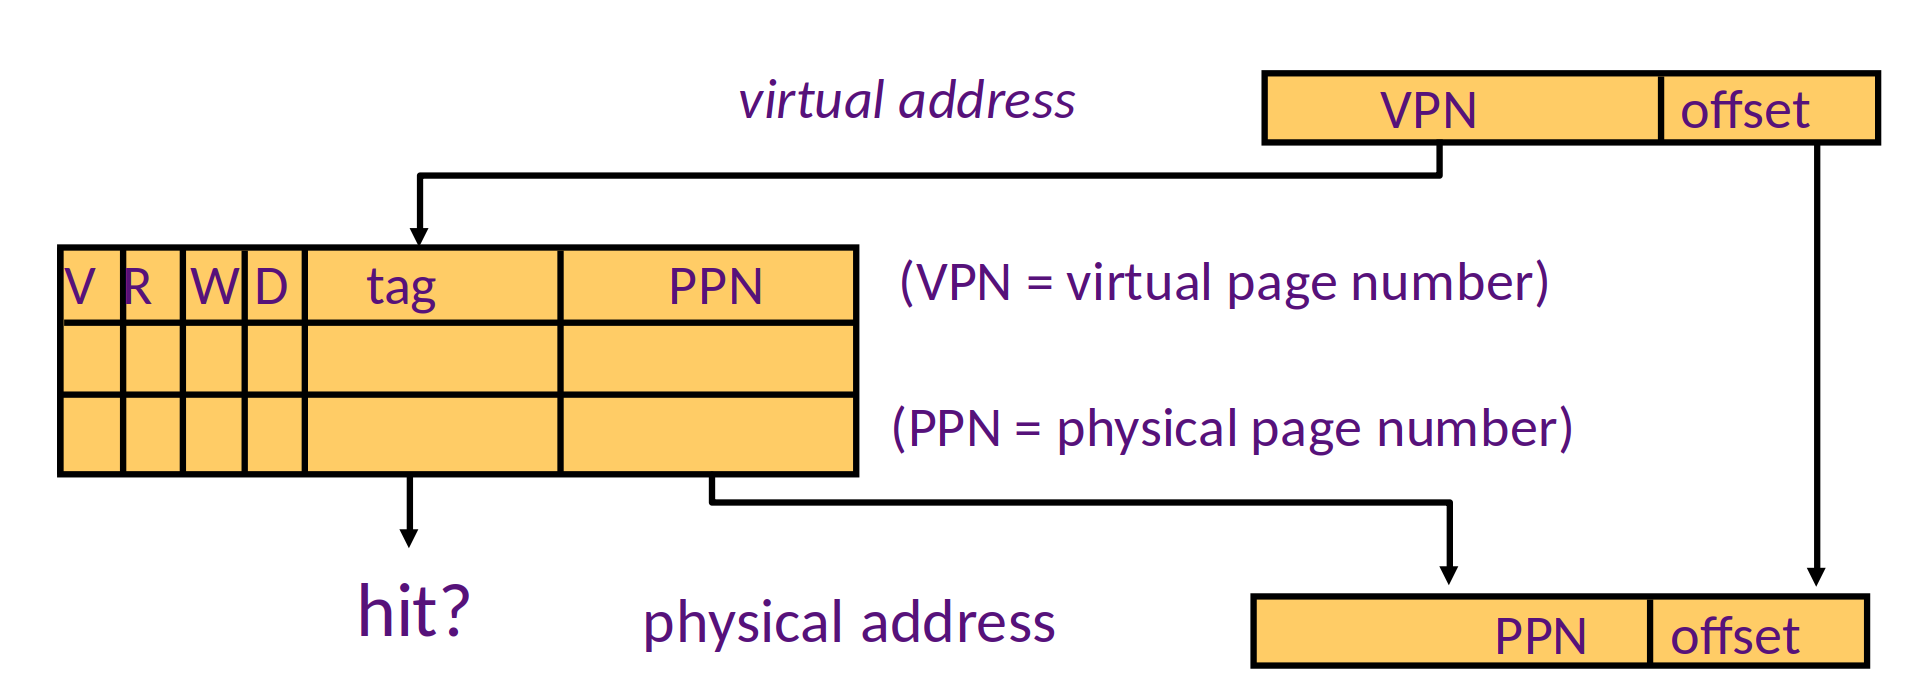
\includegraphics[width=1\linewidth]{tlb}
		\caption{TLB}
	\end{figure}
	% CS152-berkeley L08-AddressTranslation
	% 体系结构需要易于编程/编译/链接,易于软件管理	
	
\end{frame}

\begin{frame}[plain]
	
	\frametitle{虚拟内存}
	
	\begin{figure}
		\centering
		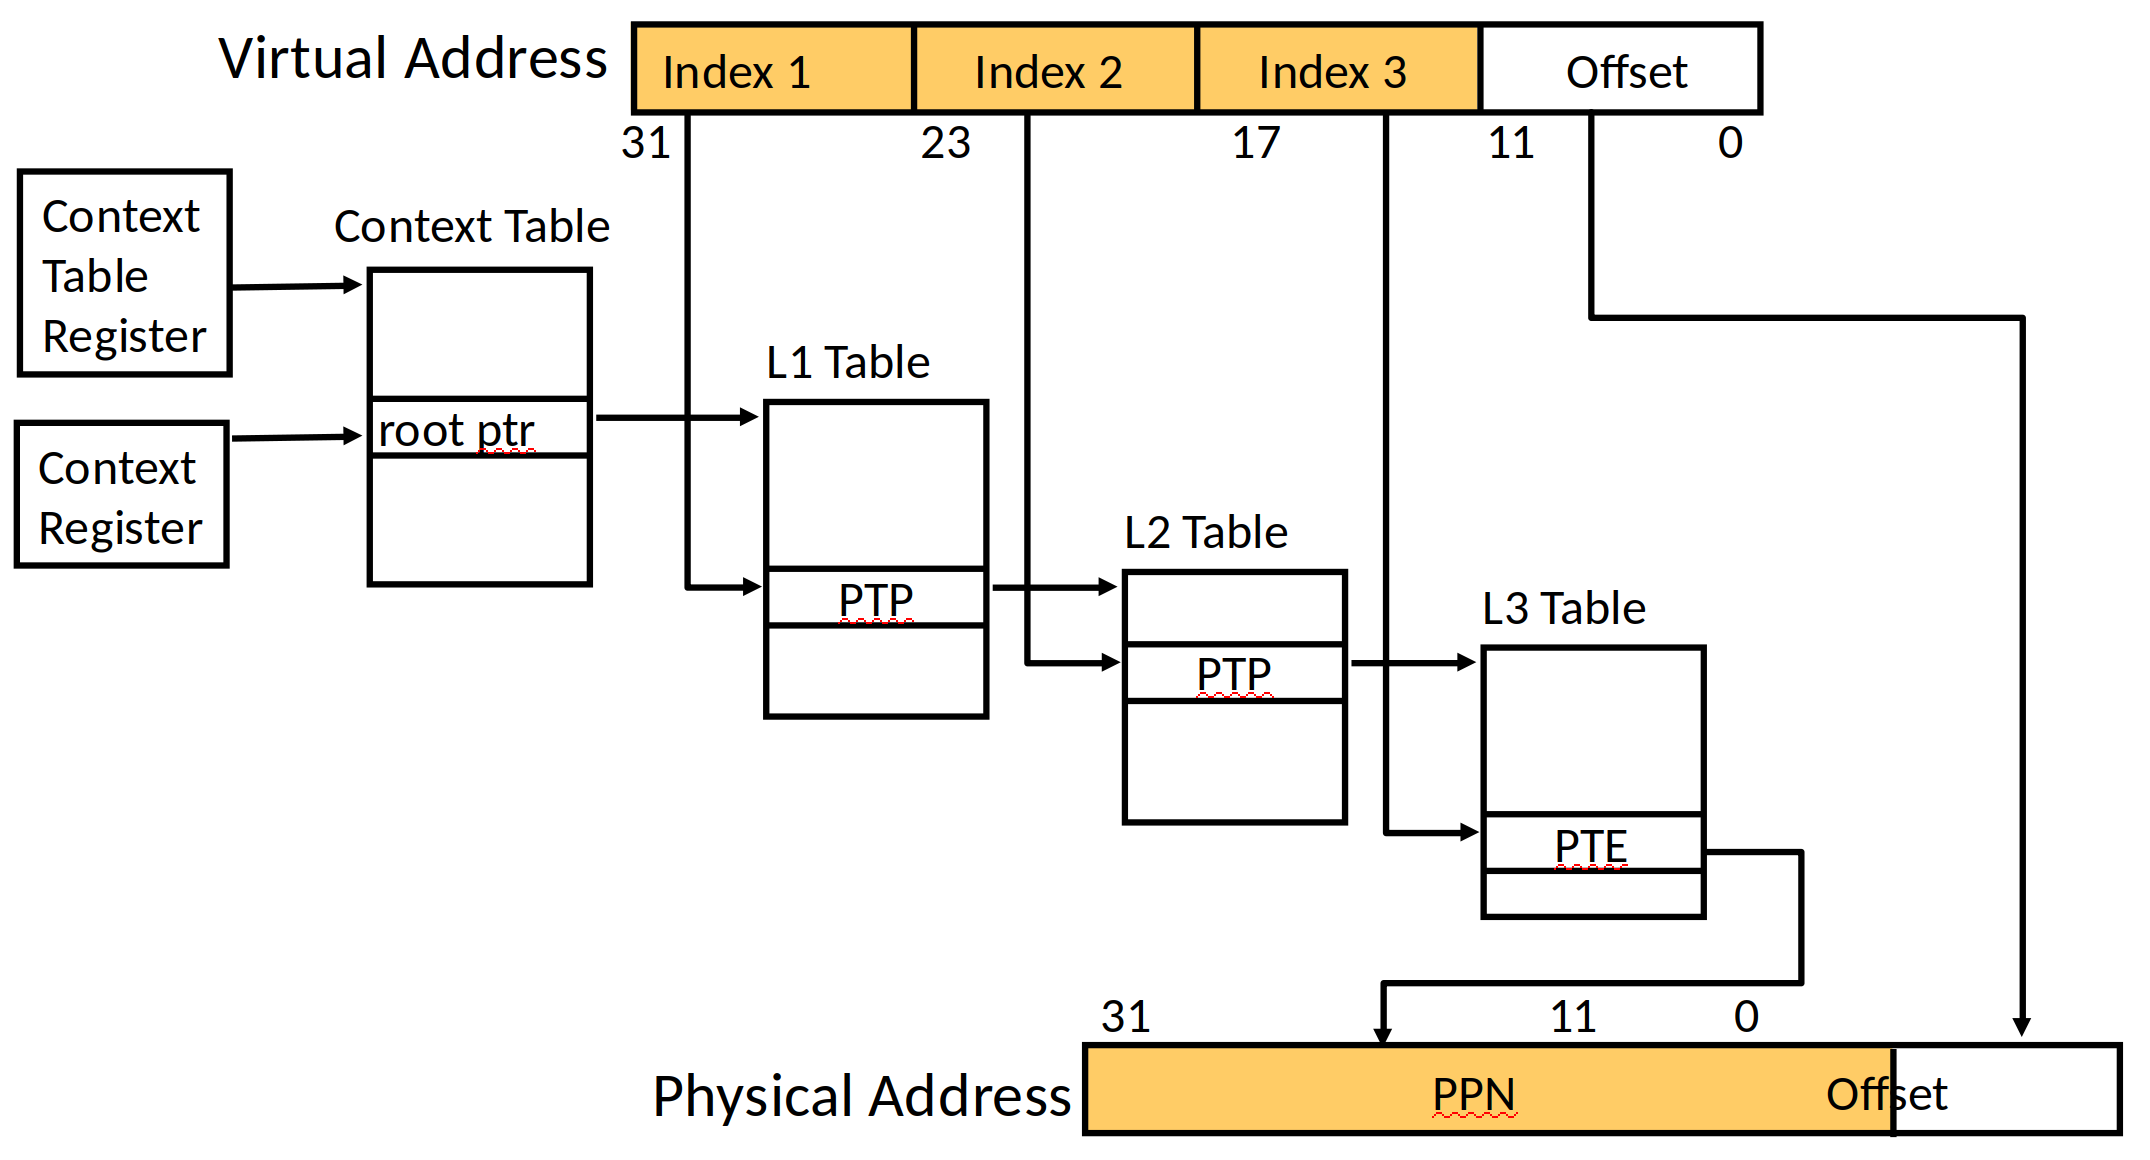
\includegraphics[width=0.75\linewidth]{mmu}
		\caption{MMU处理TLB Missing}
	\end{figure}
	% CS152-berkeley L08-AddressTranslation
	% 体系结构需要易于编程/编译/链接,易于软件管理	
	
\end{frame}

\begin{frame}[plain]
	
	\frametitle{虚拟内存}
	
	\begin{figure}
		\centering
		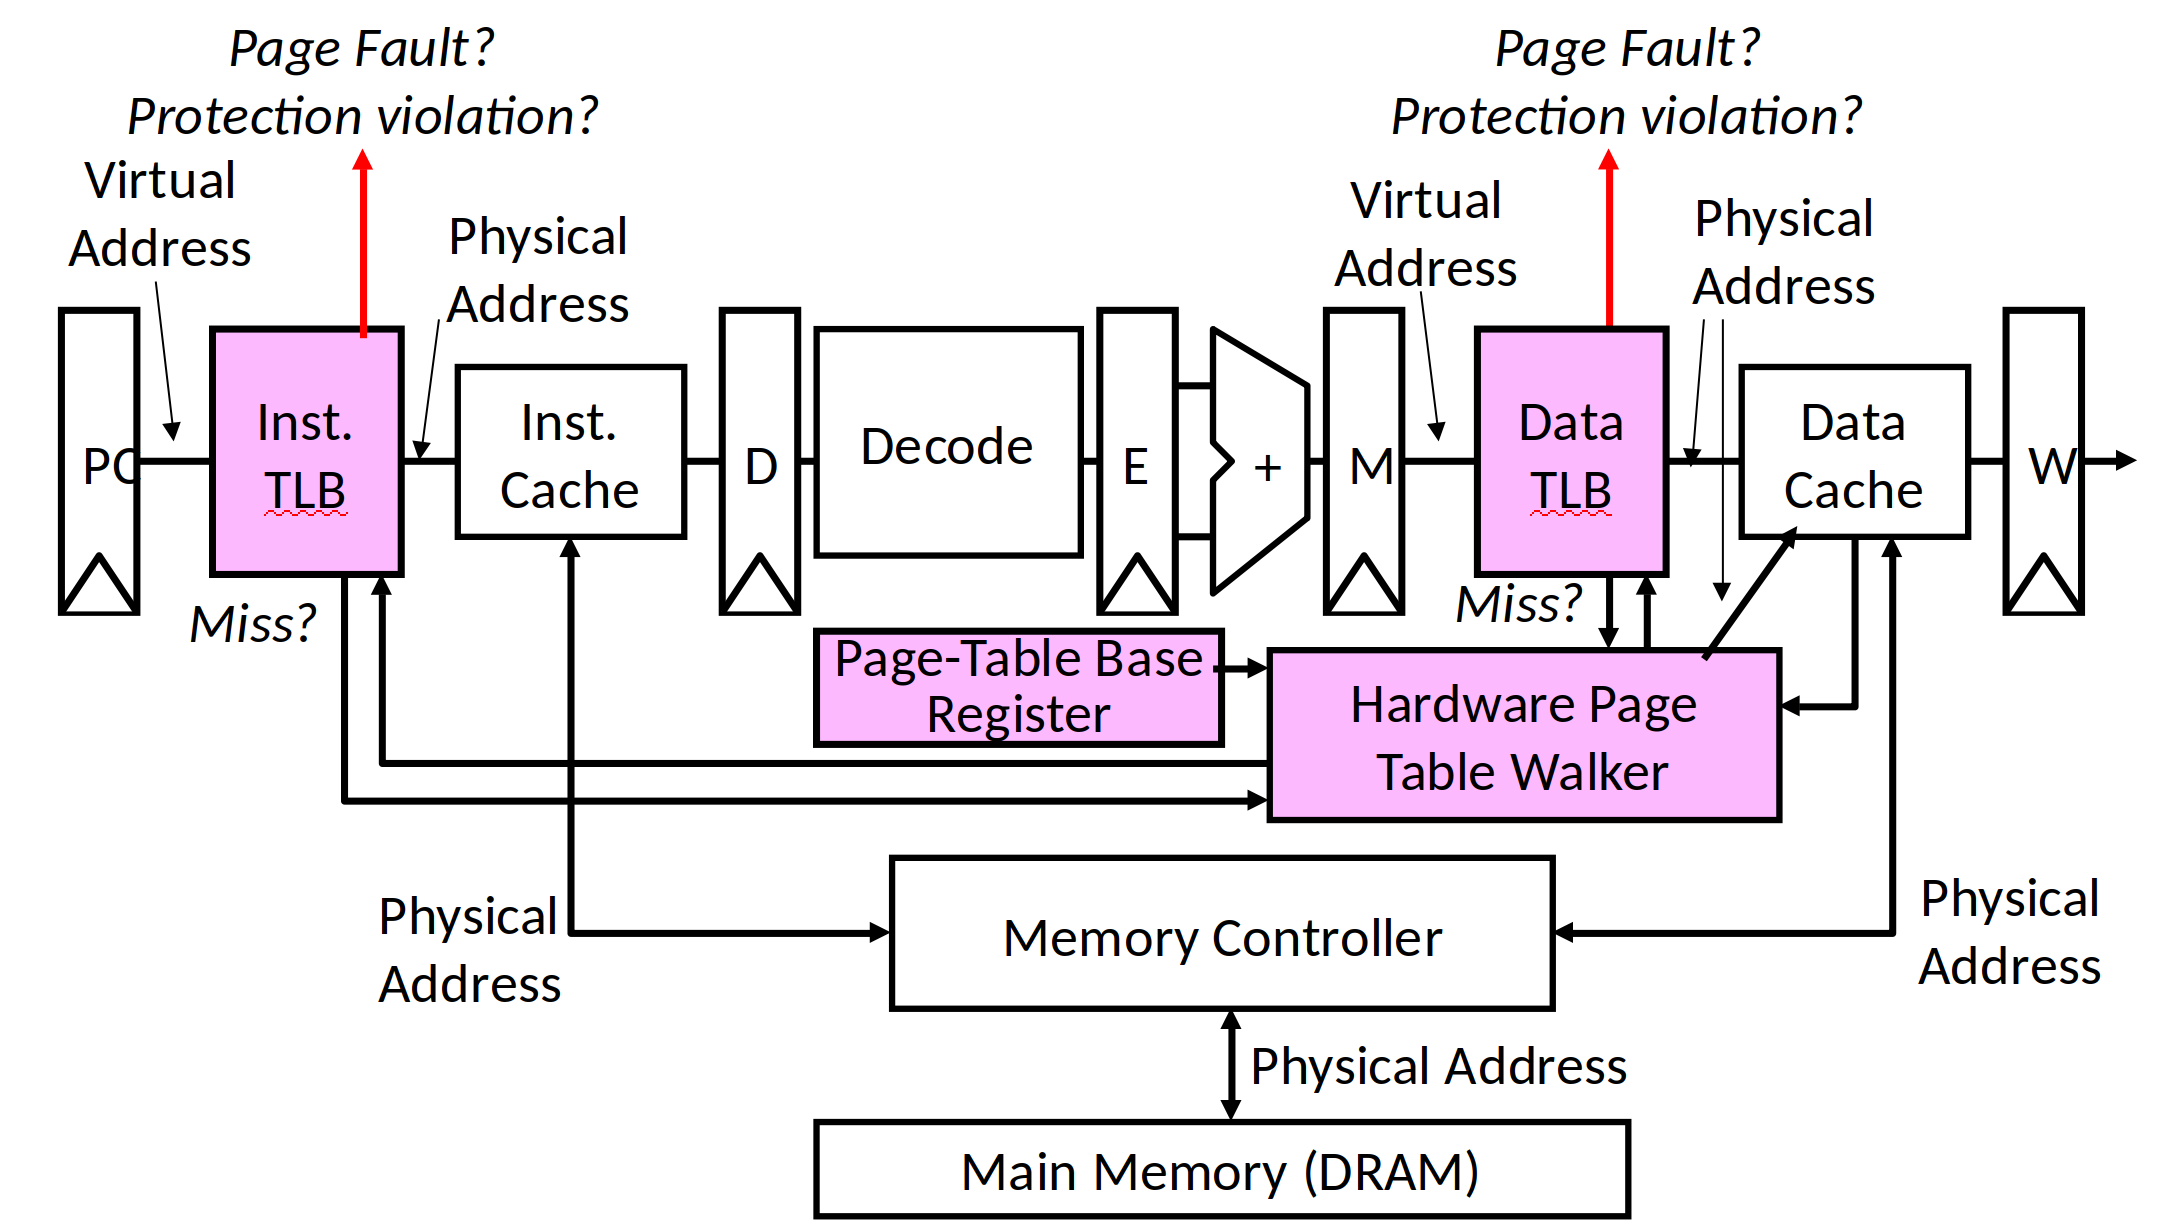
\includegraphics[width=0.8\linewidth]{arch-with-tlb-mmu}
		\caption{带MMU/TLB的计算机系统}
	\end{figure}
	% CS152-berkeley L08-AddressTranslation
	% 体系结构需要易于编程/编译/链接,易于软件管理	
	
\end{frame}

\subsection{特权模式/中断}

\begin{frame}
	\frametitle{特权模式}
	\begin{itemize}
		\item CPU硬件支持不同的特权模式
		\begin{itemize}
			\item \textbf{Kernel Mode} vs \textbf{User Mode}
			\item \textbf{Kernel Mode}可以执行\textbf{User Mode}无法执行的特权操作
			\begin{itemize}
				\item 访问外设
				\item 配置地址空间(虚拟内存)
				\item 读/写特殊系统级寄存器
			\end{itemize}			
			
			\item OS kernel运行在\textbf{Kernel Mode} 
			\item 应用程序运行在\textbf{User Mode}
			\item 每个重要的微处理器都有类似的用户/内核模式标志
				
		\end{itemize}
	\end{itemize}
\end{frame}

\begin{frame}
	\frametitle{中断机制}
	\begin{itemize}
		\item CPU硬件支持中断/异常的处理
		\item 中断是异步发生,是来自处理器外部的I/O设备的信号的结果。
		\begin{itemize}
			\item 硬件中断不是由任何一条专门的CPU指令造成,从这个意义上它是异步的。
			
		\end{itemize}
\pause
			\item 硬件中断的异常处理程序通常称为中断处理程序(interrupt handle)
			\begin{itemize}
				\item I/O设备通过向处理器芯片的一个引脚发信号,并将异常号放到系统总线上,以触发中断;
				\item 在当前指令执行完后,处理器从系统总线读取异常号,保存现场,切换到Kernel Mode;
				\item 调用中断处理程序,当中断处理程序完成后,它将控制返回给下一条本来要执行的指令。
			\end{itemize}			
\pause
			\item Timer可以稳定定时地产生中断
			\begin{itemize}
				\item 防止应用程序死占着CPU不放
				\item 让OS kernel能周期性地进行资源管理
			\end{itemize}				
	\end{itemize}
\end{frame}

%----------------------------------------------------------------------------------------

\end{document}
